\chapter{Results: DFT Reference Database}

\begin{changemargin}{1.0cm}{1.0cm}
\abstractpreamble{}
\end{changemargin}



While computer technology has advanced almost inaccordance with Moore's law, the calculations involved to approximately simulate simple structures with Quantum Mechanics are barely accessible.  Ideally, crystal structures with several hundred atoms, containing Iron, Chromium, Nickel and Palladium would have been used to derive a potential describing all four elements.  The computer used did not have the resources required for such calculations.

The model was simplified to Iron-Palladium, and the ferromagentism and antiferromagnetism of Iron and Chromium were explored using collinear spin DFT calculations.

\section{QECONVERGE}

\subsection{Purpose of Code}

A code was developed to automate the process of finding the ecutwfc and ecutrho values that bring the calculation within the desired convergence parameters.  Colour plots of Ecutwfc and Ecutrho against energy and force are created to assist the user in visualising the results.  Similar plots of smearing amount and k-points vs energy and force are also created to allow the user to pick values within the desired convergence amount.


\subsection{Source Code and Instructions}

The source code and instructions on how to use the program are available to download from GitHub.

https://github.com/BenPalmer1983/qeconverge




\section{Convergence of Key DFT Settings and Testing}

\subsection{Introduction}

Prior to generating a database of atom configurations, calculated forces, stresses and energies, key DFT settings needed to be selected and tested.  The Python code Qeconverge was written and used to converge the ecutwfc, ecutrho, k-points and degauss smearing values for each of the pseudopotentials required.  

The following pseudo-potential files were used for each element:



\begin{itemize}
\item Aluminium: a plane wave GGA potential Pd.pbe-spn-kjpaw\_psl.1.0.0.UPF
\item Chromium: a plane wave GGA potential Cr.pbe-spn-kjpaw\_psl.1.0.0.UPF
\item Iron: a plane wave GGA potential Fe.pbe-spn-kjpaw\_psl.1.0.0.UPF 
\item Palladium: a plane wave GGA potential Pd.pbe-spn-kjpaw\_psl.1.0.0.UPF
\end{itemize}


For each pseudo-potential, the ecutwfc, ecutrho and kpoint and degauss settings were converged.  Ideally, the k-points settings would have been increased, but doing so would have been prohibitive due to the amount of time taken to perform each calculation.

By the time calculations were being executed for a 32 atom supercell, one node of 20 processor cores would run for several days up to a week or more, requiring the calculation to be submitted to continue multiple times.  Aluminium is also considered in the results section, as it is a simpler atom to run trial calculations with, and to compare to experimental results.



\subsection{Collinear Spin Calculations for Iron}

The relaxed crystal lattice parameters were calculated for iron, chromium and palladium.  Chromium will not be used in the Fe-Pd fitting calculations.  However, there is a large increase in computation time between non-spin and collinear spin calculations.  The ferromagnetic structure of BCC iron, antiferromagnetic structure of FCC iron and BCC chromium were investigated.

\begin{table}[h]
\begin{center}
\begin{tabular}{c c c c c c}
\hline
Description & A0 (ang) & V0 (bohr3) & B0 (GPA) & E0 (Ry) (DFT Only) \\
\hline \\
Exp. & 2.91 & 83.23 & 160 & - \\
AFM & 2.86 & 78.768 & 217 & -248.2216 \\
FM & 2.85 & 78.102 & 267 & -248.2214 \\
No Mag & 2.85 & 78.102 & 267 & -248.2214 \\
\end{tabular}
\end{center}
\caption{Chromium properties with and without collinear spin}
\end{table}

The DFT calculated values for the bulk modulus were larger than expected, but the anniferromagnetic calculation was much closer to the experimental value.  The E0 values do not reflect the actual energies, but show the relative calculated values.  The antiferromagnetic configuration gives the lowest, optimum, energy.


\begin{center}
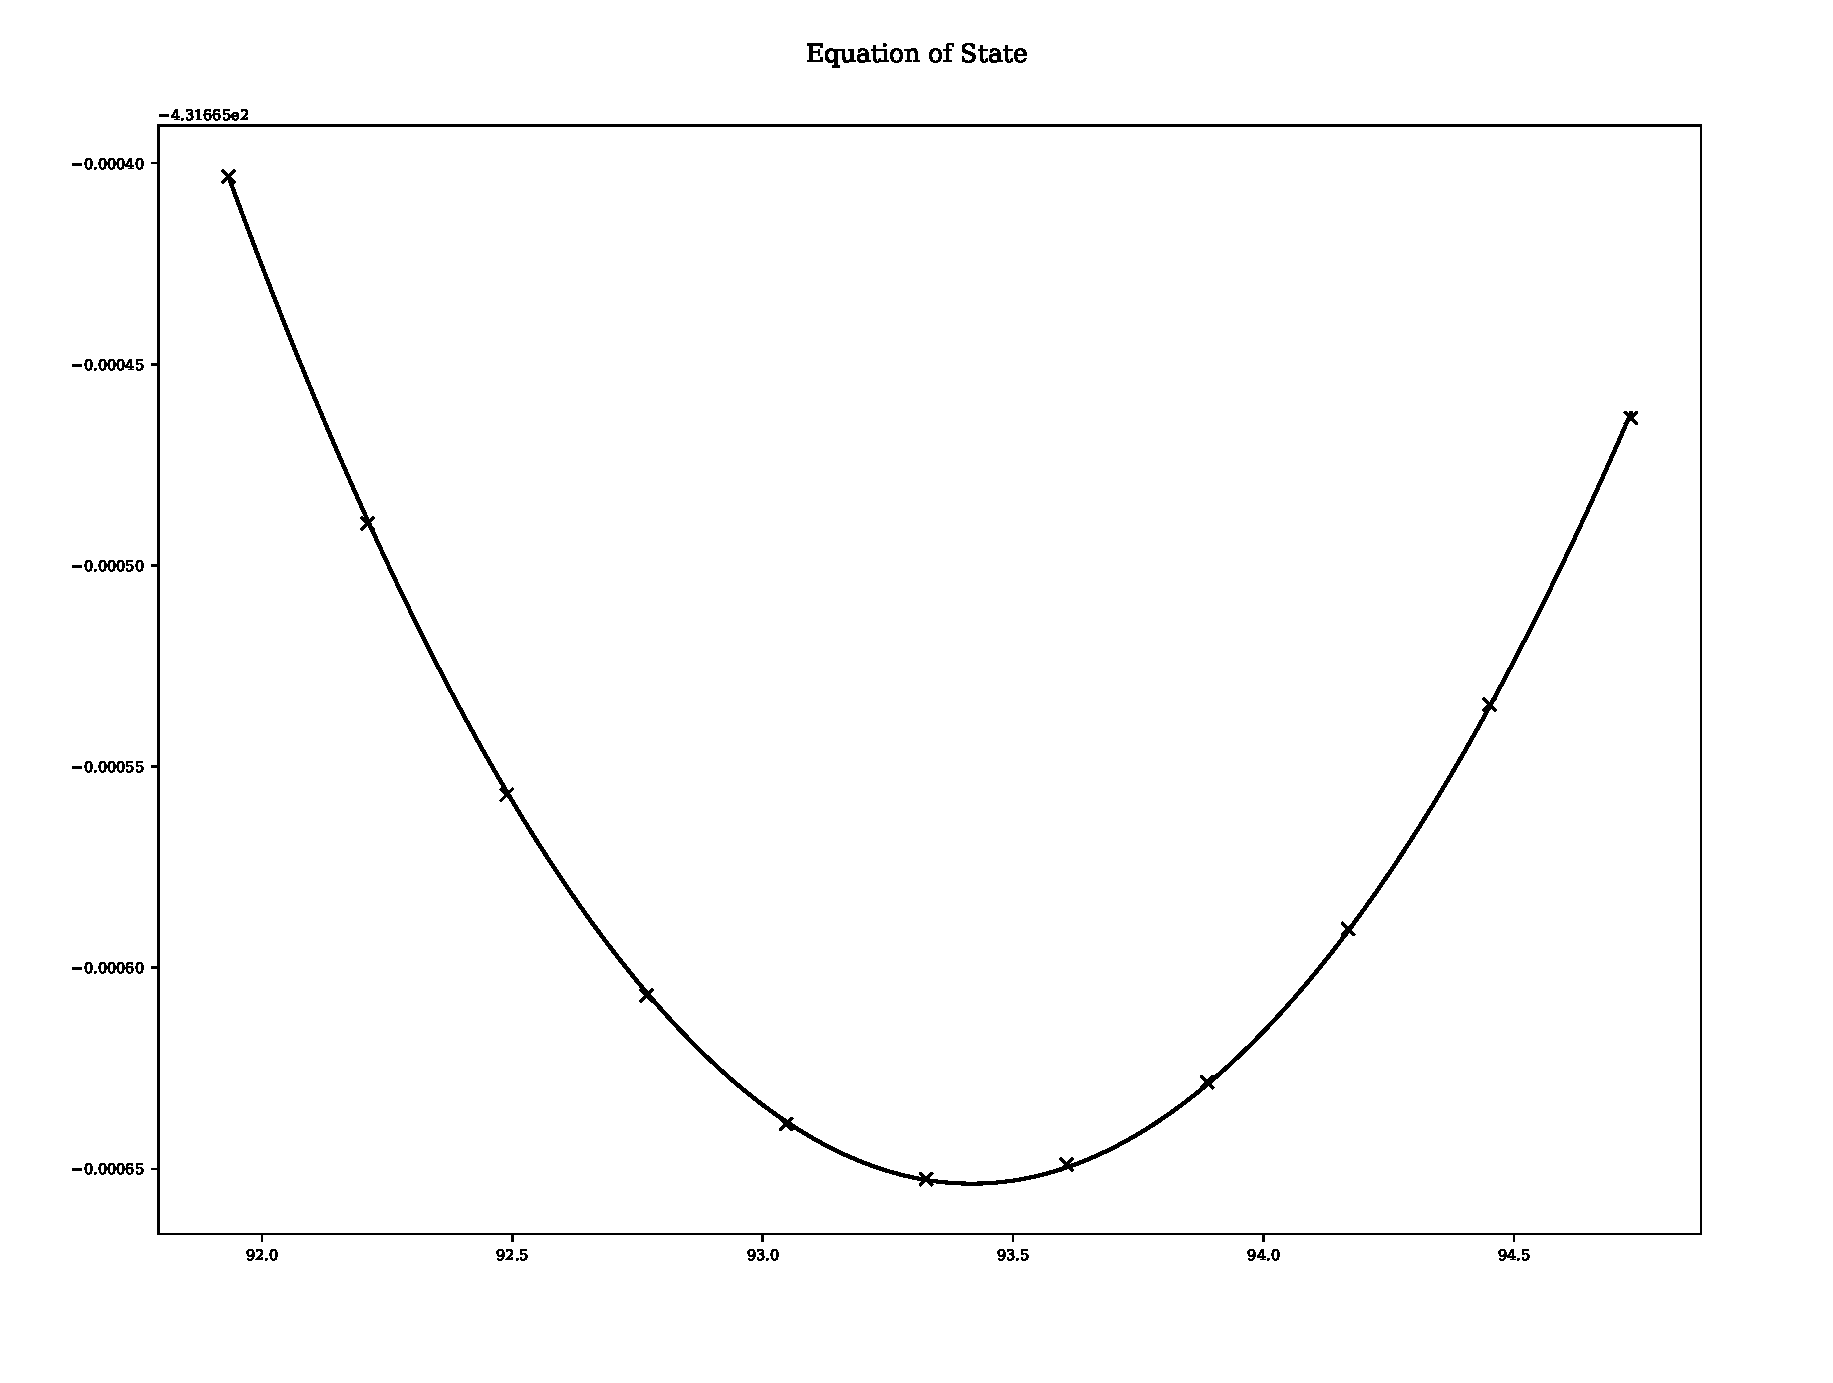
\includegraphics[scale=0.35]{chapters/results_dft_reference_db/qeeos_plots/cr-mag/eos.eps}
\end{center}






\subsection{Convergence Results}


\begin{table}[h]
\begin{center}
\begin{tabular}{c c c c c c}
\hline
Element & Pseudopotential & Ecutwfc & Ecutrho & K-points & Degauss \\
\hline \\
Al & Al PBE KJPAW & 50 & 200 & 11 & 0.04 \\
Fe & FE PBE KJPAW & 71 & 431 & 9 & 0.04 \\ 
Pd & FE PBE KJPAW & 71 & 431 & 9 & 0.04 \\ 
\end{tabular}
\end{center}
\caption{DFT Settings}
\end{table}




\subsubsection{Aluminium}






\subsubsection{Iron}




\subsubsection{Palladium}



\subsubsection{Iron-Palladium}





\begin{figure}[h]
  \begin{center}
    \includegraphics[scale=0.55]{chapters/results_dft_reference_db/qeconverge/pd_interpolated_summary_colour.eps}
    \caption{Palladium Convergence Calculations}
    \label{graph:graph1}
  \end{center}
\end{figure}



\section{Computer Package Development}
 
<Intro>





\section{QEEOS}

\subsection{Purpose of Code}

A code was developed to automate the process of calculating the equation of state and elastic constants of a material using Quantum Espresso.  It requires an input file and a starting PWscf input file.  

\begin{itemize}
\item the input configuration is relaxed using the vc-relax option in PWscf
\item configuration files are created to compute the equation of state, and PWscf is used to calculate the energies of these configurations
\item to compute the elastic constants, nine distortions are applied to the relaxed configuration with the required number of steps for each strain applied to each distortion, and these are processed with PWscf
\item once all DFT work has completed, the Birch-Murnaghan equation of state is fit to the first set of energies, and the nine orthorhombic elastic constants are fit to the results of the second set of energies
\end{itemize}


\subsection{Source Code and Instructions}

The source code and instructions on how to use the program are available to download from GitHub.

https://github.com/BenPalmer1983/qe\_eos







\begin{figure}[h]
  \begin{center}
    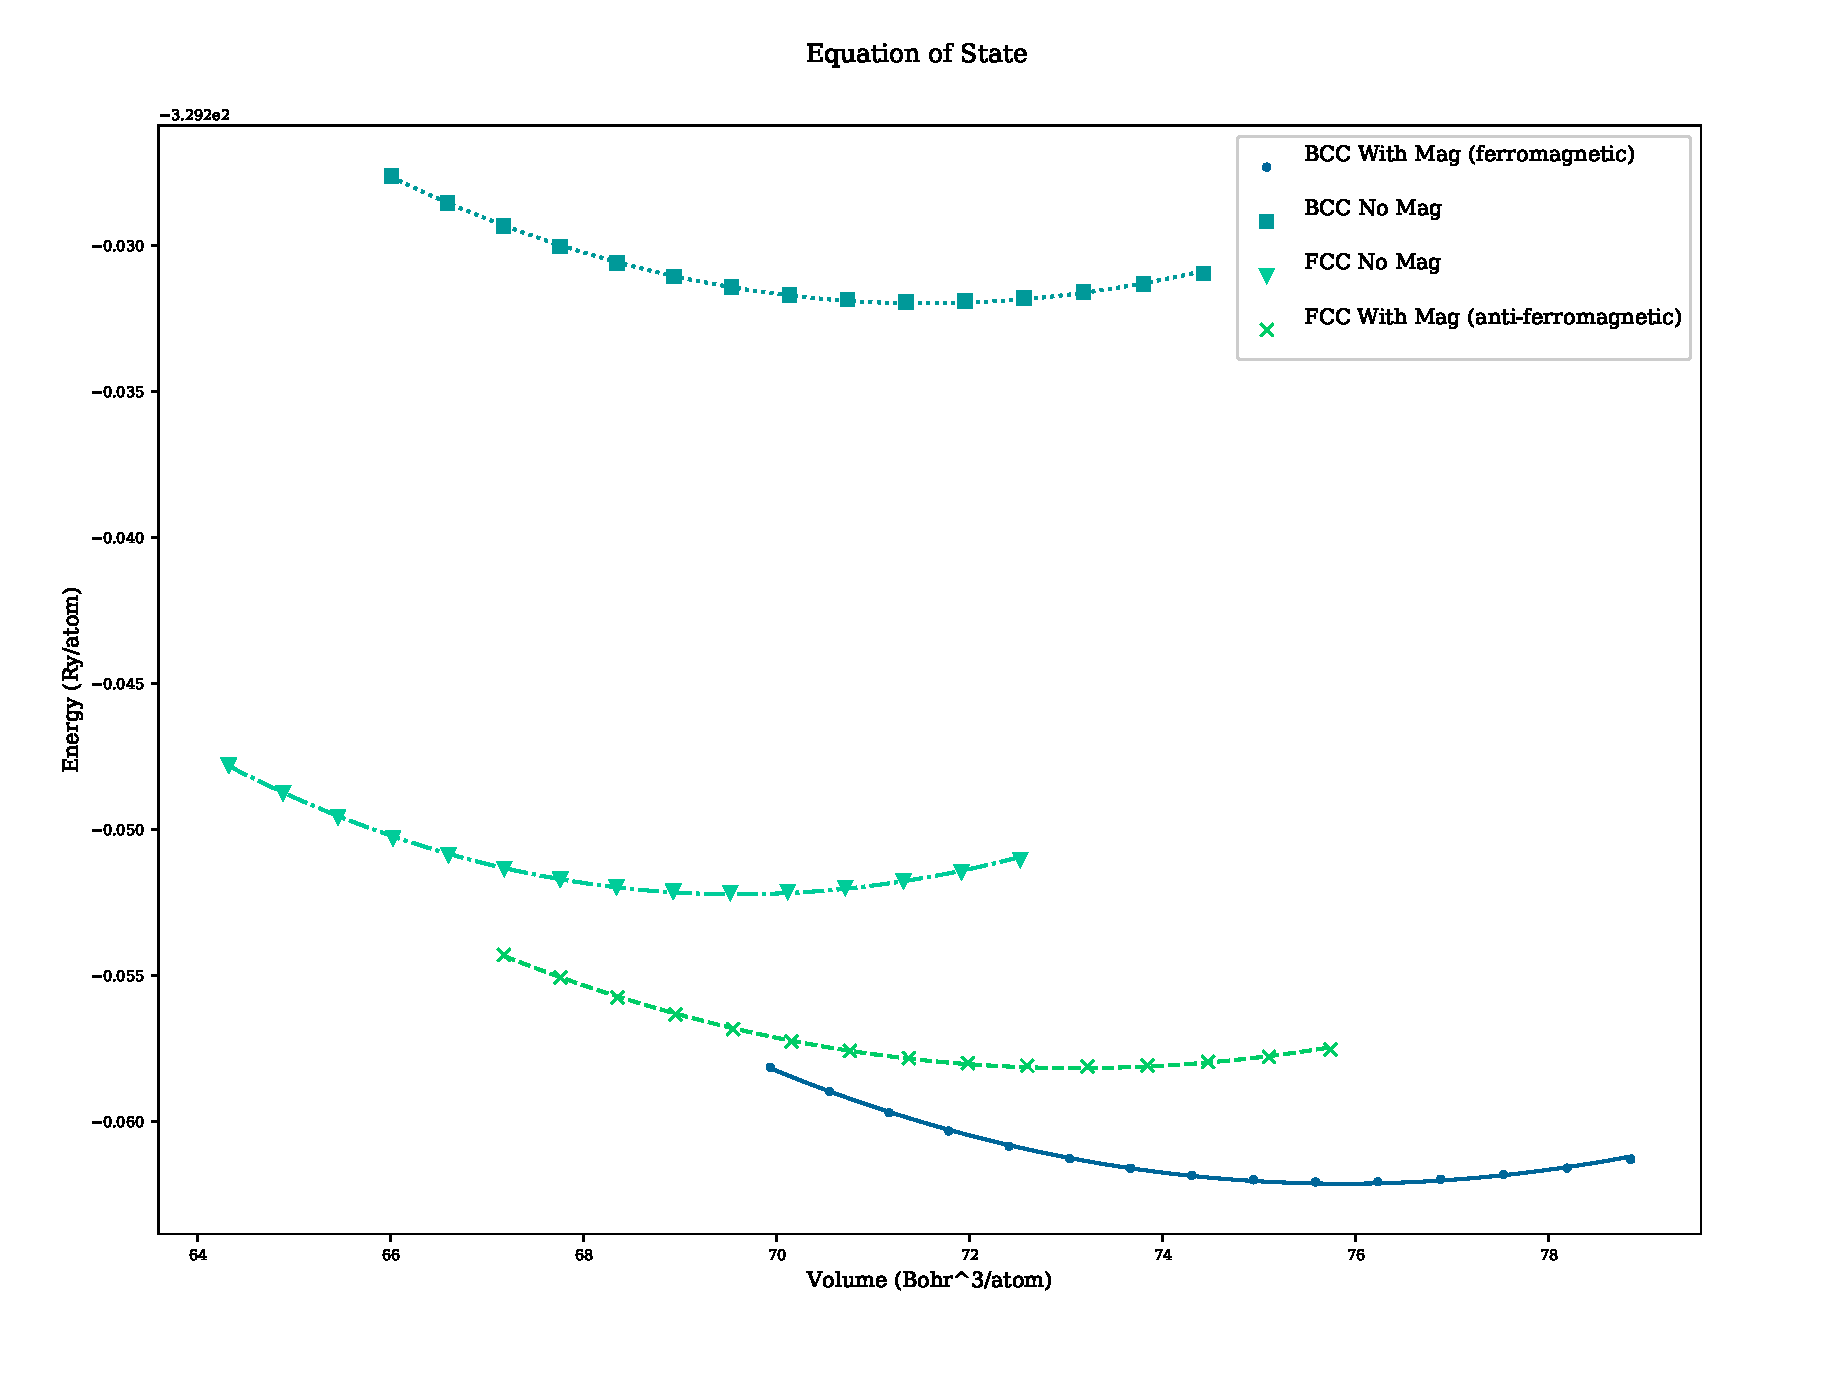
\includegraphics[scale=0.55]{chapters/results_dft_reference_db/qeeos_plots/iron_eos_comparison.eps}
    \caption{Palladium Convergence Calculations}
    \label{graph:graph1}
  \end{center}
\end{figure}






\section{EAMPA}

\subsection{Purpose of Code}

A code was developed to automate the process of calculating the equation of state and elastic constants of a material using Quantum Espresso.  It requires an input file and a starting PWscf input file.  

\begin{itemize}
\item the input configuration is relaxed using the vc-relax option in PWscf
\item configuration files are created to compute the equation of state, and PWscf is used to calculate the energies of these configurations
\item to compute the elastic constants, nine distortions are applied to the relaxed configuration with the required number of steps for each strain applied to each distortion, and these are processed with PWscf
\item once all DFT work has completed, the Birch-Murnaghan equation of state is fit to the first set of energies, and the nine orthorhombic elastic constants are fit to the results of the second set of energies
\end{itemize}


\subsection{Source Code and Instructions}

The source code and instructions on how to use the program are available to download from GitHub.

https://github.com/BenPalmer1983/qe\_eos







